%-*-coding: utf-8-*-
\chapter{Обзор предметной области}

\label{ch:review}

\section{Планирование маршрутов}

\label{sec:path-planning}

Задача планирования маршрута (англ. path planning) заключается в
поиске пути из точки $A$ в точку $B$, удовлетворяющего некоторым
ограничениям. В данной работе слова «\emph{маршрут}» и «\emph{путь}»
используются взаимозаменяемо. При планировании маршрута по воде
ограничениями являются полигональные препятствия (материки, острова и
так далее), которые запрещено пересекать. Стандартный способ решения
этой задачи состоит в построении графа, вершины которого соответствуют
некоторым точкам в мире, а ребро между двумя вершинами может
присутствовать в графе только при условии, что оно не пересекает ни
одно из препятствий, и поиске кратчайшего пути в этом графе.
Известно~\cite{visibility-proof}, что любой кратчайший путь между
двумя вершинами представляет из себя ломаную, вершины которой являются
вершинами препятствий. Потому для поиска кратчайшего пути требуется
построить \emph{граф видимости}.

\emph{Граф видимости (англ. visibility graph)} --- граф, вершины
которого являются вершинами полигональных препятствий, а ребро между
вершинами $u$ и $v$ принадлежит графу тогда и только тогда, когда
отрезок $uv$ не пересекает ни одно препятствие.

Таким образом, любой кратчайший путь между двумя точками является
кратчайшим путём в графе видимости и может быть найден с помощью
любого алгоритма поиска кратчайшего пути в графе. Одними из наиболее
популярных алгоритмов являются алгоритм
Дейкстры~\cite{dijkstra1959note} и $A^*$~\cite{hart1968formal}. Стоит
отметить, что довольно часто не требуется находить кратчайший маршрут,
достаточно найти какой-нибудь корректный маршрут, желательно близкий к
кратчайшему. В этом случае используется \emph{навигационный граф}.

\emph{Навигационный граф} --- граф, построенный по полигональным
препятствиям, вершины которого соответствуют некоторым точкам в
пространстве, а ребро между вершинами $u$ и $v$ может принадлежать
графу только тогда, когда отрезок $uv$ не пересекает ни одно
препятствие.

Как было отмечено во введении, задача планирования единственного
кратчайшего пути имеет множество недостатков при поиске маршрутов по
воде. Поэтому возникает задача поиска семейств маршрутов. Данная
задача исследована не так хорошо, как планирование единственного
маршрута, однако известны различные алгоритмы, обзор которых приведён
в следующем разделе~(\ref{sec:existing-algos}). При поиске семейств маршрутов по воде естественно
требовать, чтобы все маршруты были, неформально говоря, попарно
непохожи, отличаясь способом обхода существенных препятствий.
Например, на рисунке \ref{fig:similar-paths} маршруты не имеют общих
рёбер, но являются очень похожими. В то же время на рисунке
\ref{fig:dissimilar-paths} представлены непохожие маршруты, поскольку
то, с какой стороны обходится остров, может быть достаточно
существенно. Более наглядно неформальное описание похожести маршрутов
проиллюстрировано на рисунках \ref{fig:similar-paths2} и \ref
{fig:dissimilar-paths2}.

\begin{figure}
    \centering
    \begin{minipage}{.5\textwidth}
        \centering
        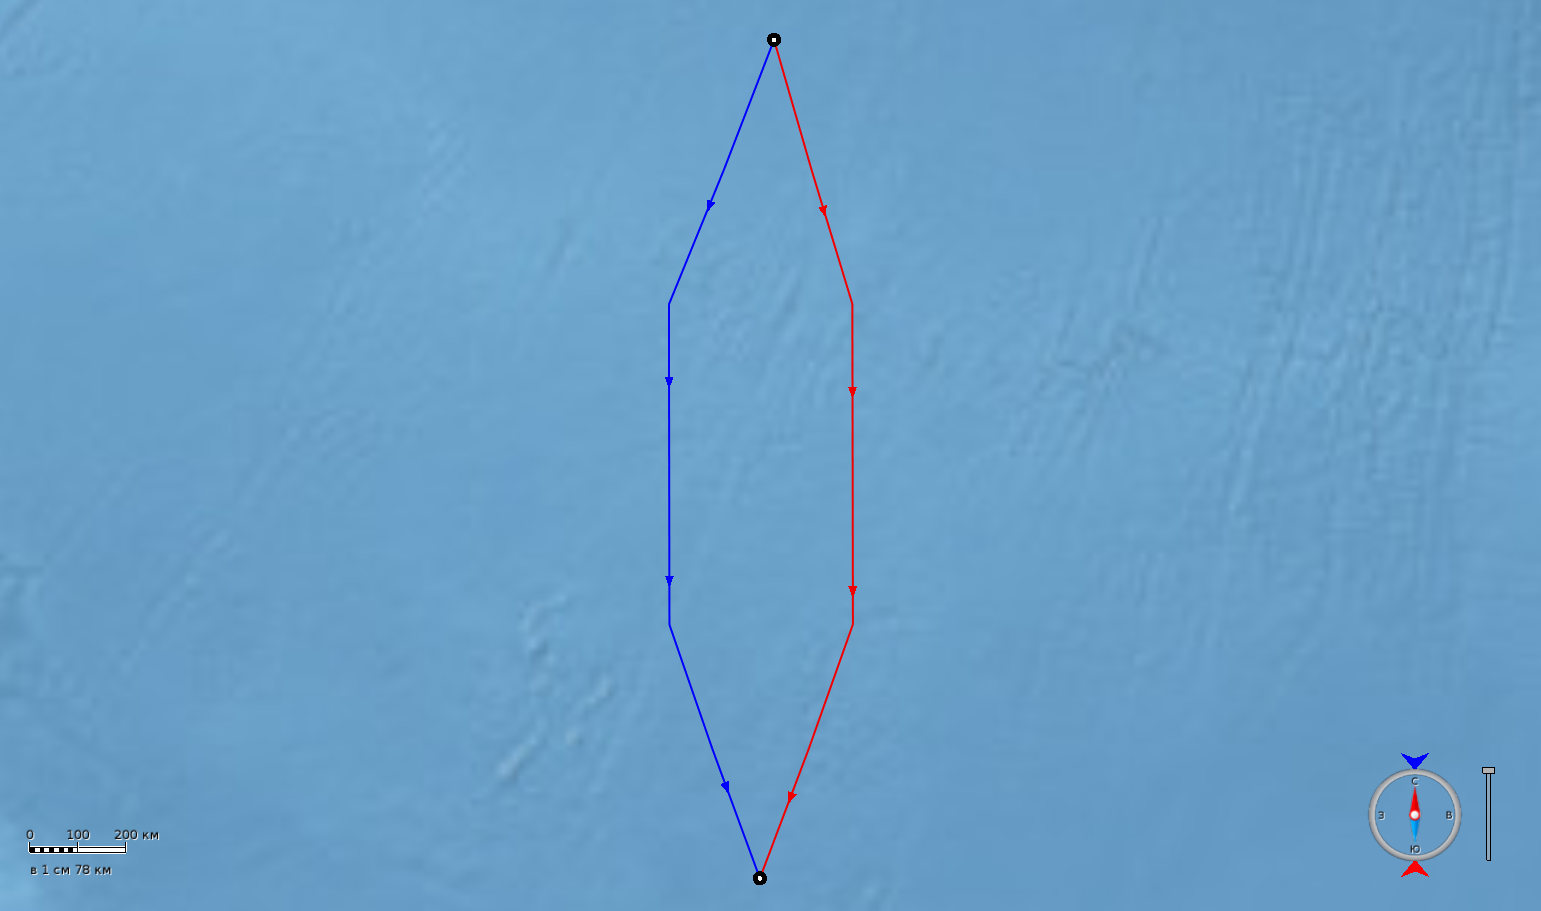
\includegraphics[width=\textwidth, clip=true, trim = 300 0 300
        0]{Introduction/similar}
        \captionof{figure}{Похожие маршруты}
        \label{fig:similar-paths}
    \end{minipage}%
    \begin{minipage}{.5\textwidth}
        \centering
        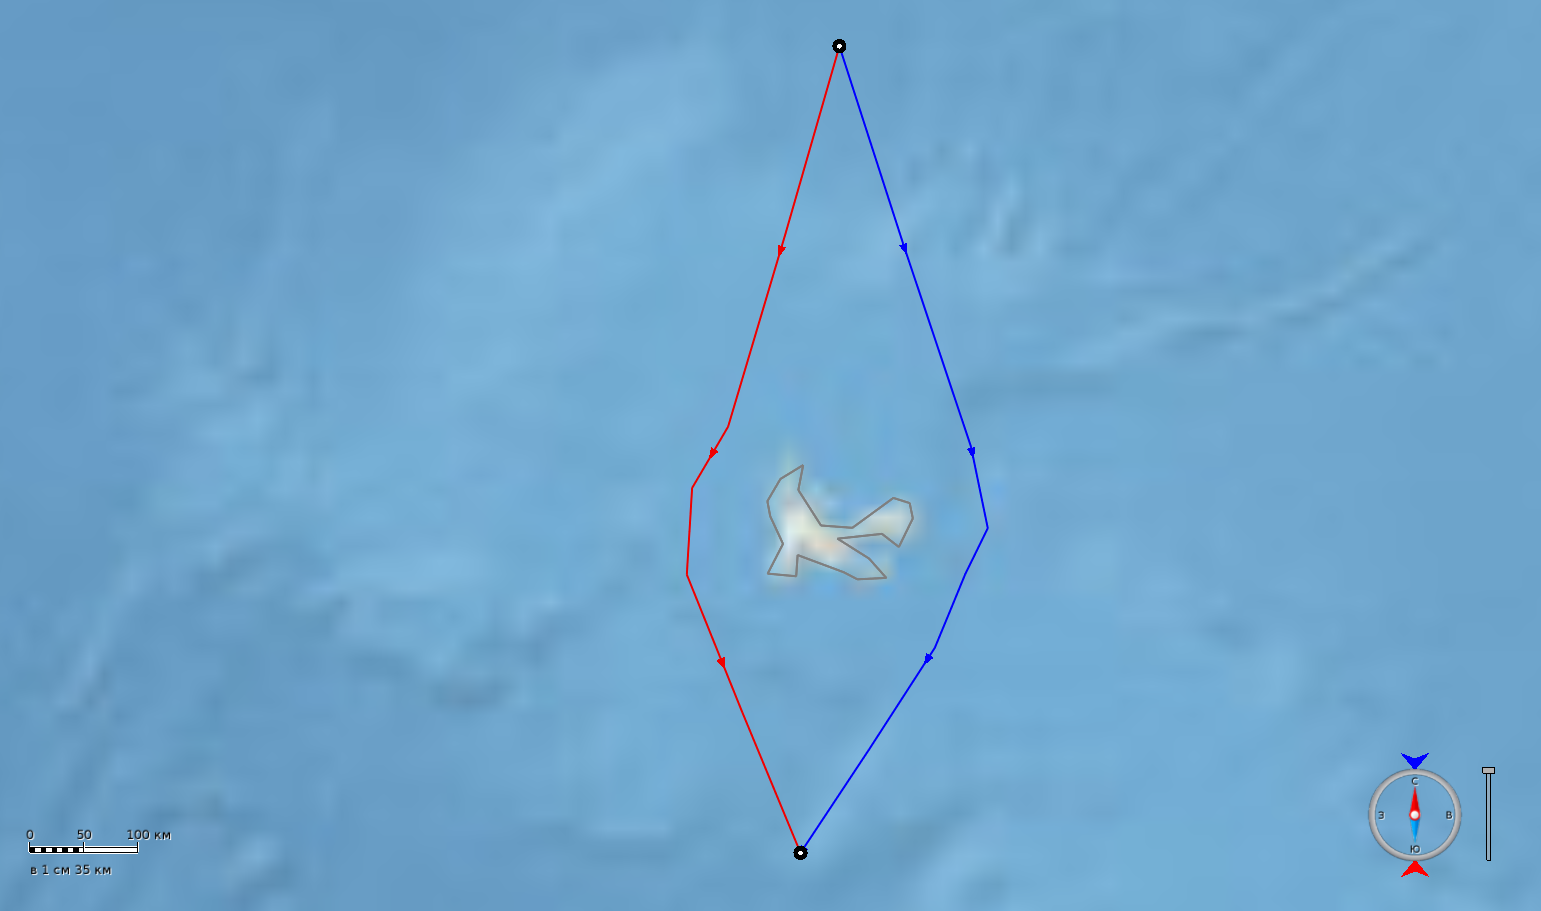
\includegraphics[width=\textwidth, clip=true, trim = 300 0 300
        0]{Introduction/dissimilar}
        \captionof{figure}{Непохожие маршруты}
        \label{fig:dissimilar-paths}
    \end{minipage}
\end{figure}

\begin{figure}
    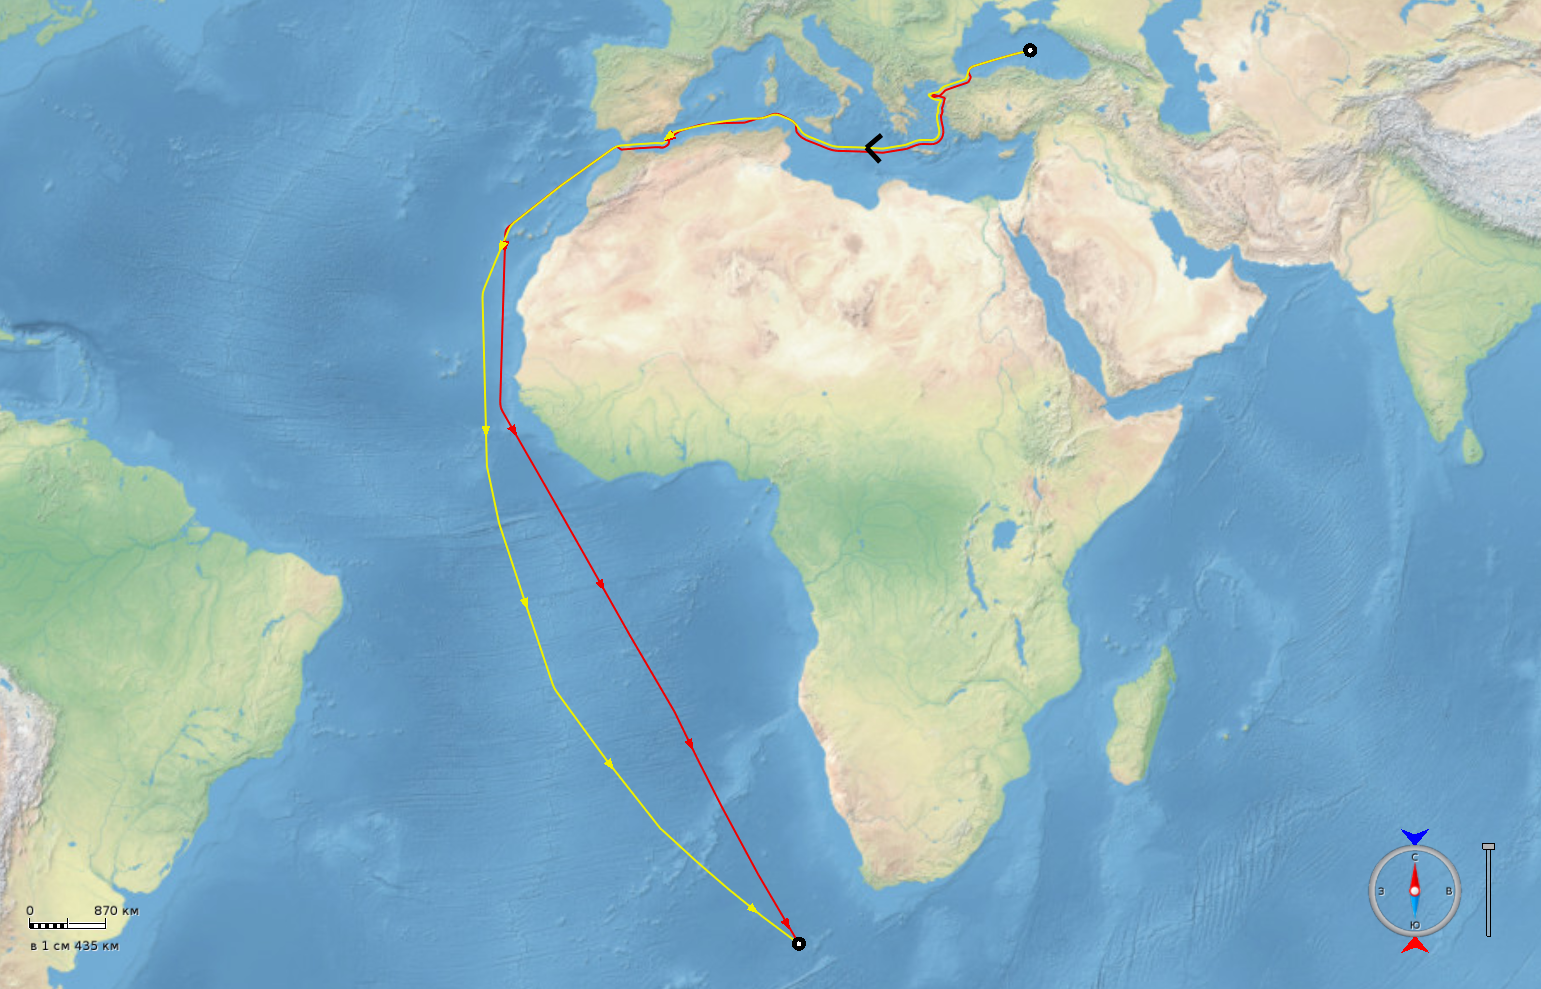
\includegraphics[width=\textwidth]{Introduction/similar2}
    \caption{Похожие маршруты}
    \label{fig:similar-paths2}
\end{figure}

\begin{figure}
    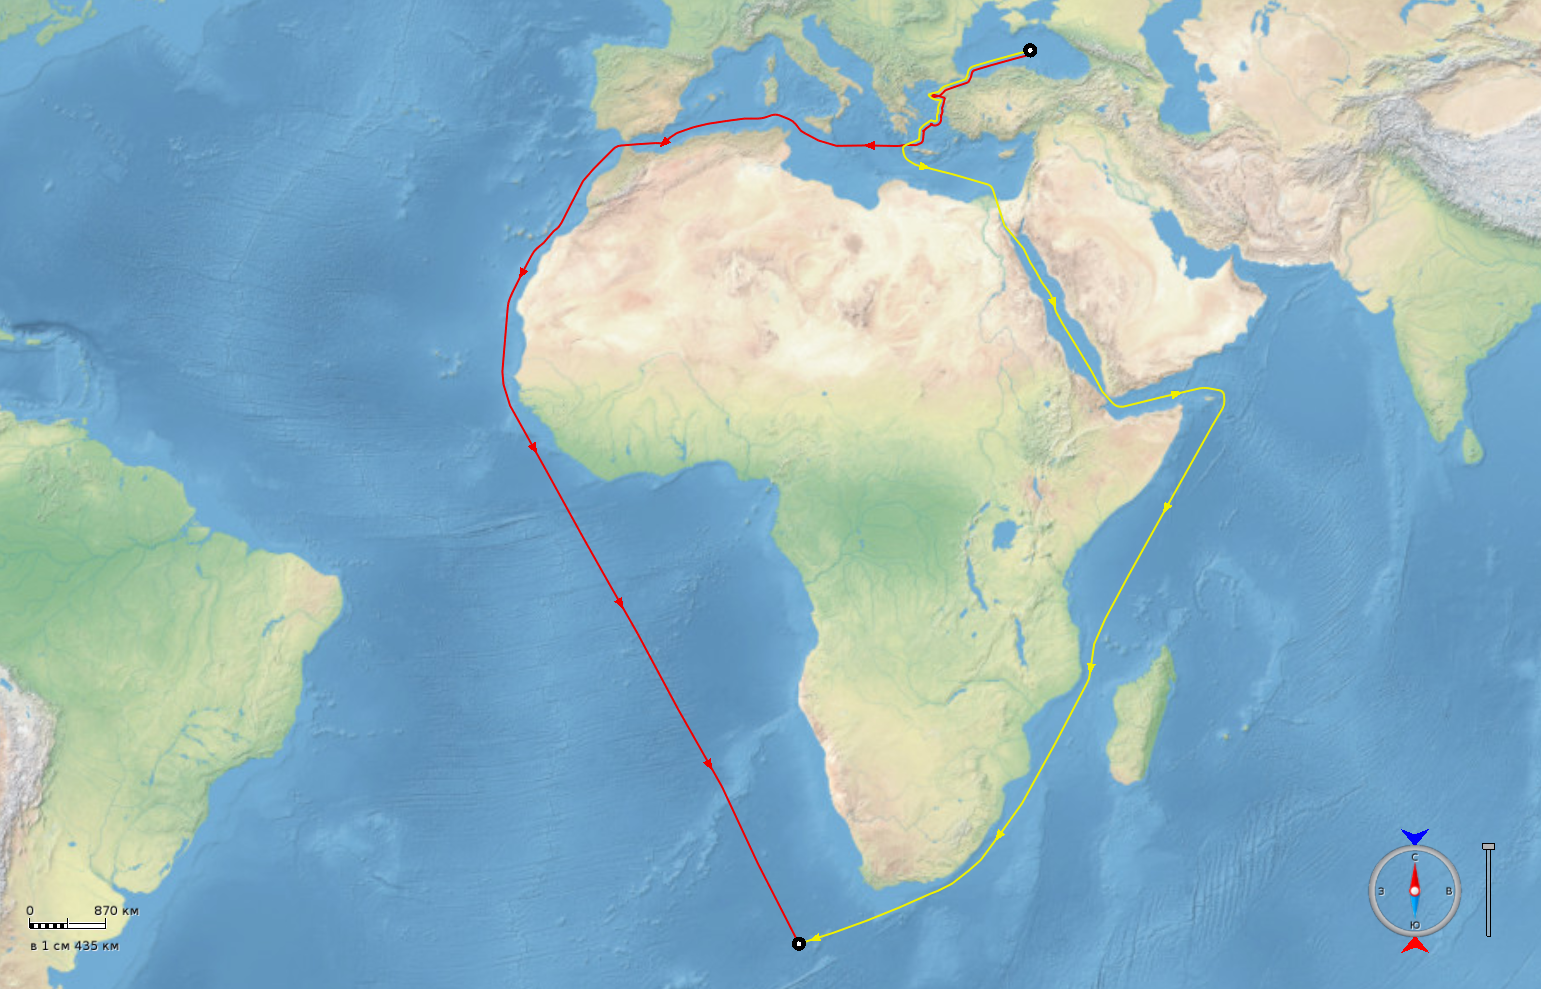
\includegraphics[width=\textwidth]{Introduction/dissimilar2}
    \caption{Непохожие маршруты}
    \label{fig:dissimilar-paths2}
\end{figure}

При решении такой задачи не следует использовать граф видимости по
трём причинам:
\begin{enumerate}
    \item Граф видимости позволяет найти кратчайший путь на плоскости,
      однако Земля не плоская, поэтому кратчайший путь в графе
      видимости не обязан являться кратчайшим маршрутом между двумя точками.
    \item Данная задача выполняет поддержку принятия решения,
      заключающуюся в предложении альтернативных маршрутов, которые
      могут быть выбраны пользователем. При этом небязательно находить
      строго кратчайший путь, поскольку решение задачи в любом случае
      не является окончательным результатом.
    \item В графе видимости, построенном по контурам, взятым с
      мелкомасштабной морской навигационной карты, будет слишком много
      рёбер, из-за чего поиск может выполняться неприемлимо долго.
\end{enumerate}
Поэтому для поиска используется навигационный граф, построение и
структура которого описаны в главе~\ref{ch:theoretical-solution}.

\FloatBarrier

\section{Существующие алгоритмы поиска семейств маршрутов}

\label{sec:existing-algos}

Известно множество подходов к проблеме поиска семейств
маршрутов~\cite{lim2005shortest, dial1971probabilistic, mafast}.
Однако они обладают следующими недостатками:
  
\begin{itemize}
    \item Все решения разрабатывались для других целей. Например, для
      поиска маршрутов по дорогам или в транспортных сетях. В этих
      случаях имеется граф дорог, в котором осуществляется поиск путей.
      Если два пути имеют мало общих рёбер, то они, как правило, имеют
      существенные различия. В то же время два маршрута по воде, не
      имеющие общих рёбер, могут проходить по одним и тем же морям и
      каналам.
    \item Предложенные алгоритмы работают с довольно абстрактными
      графами и не учитывают привязанность вершин к реальным координатам
      в мире.
    \item Следствием первых двух пунктов является то, что при
      применении таких решений к задаче поиска семейств маршрутов
      кораблей находятся слишком похожие маршруты.
\end{itemize}

\FloatBarrier

\subsection{Lim, Kim, 2005}

\label{subsec:lim-kim}

В~\cite{lim2005shortest} описывается алгоритм поиска непохожих
маршрутов в сетях дорог. Непохожесть маршрутов является одной из
главных целей алгоритма. В качестве критерия, описывающего похожесть
маршрутов, используется отношение длины перекрывающейся части путей к
длине одного из путей (степень перекрытия). Сам алгоритм устроен
следующим образом: сначала происходит поиск кратчайшего пути в графе,
затем веса всех рёбер на этом пути увеличиваются, считается степень
перекрытия, и если она больше порогового значения, то процесс
заканчивается, иначе найденный путь добавляется в результирующее
множество, и процесс продолжается.

\begin{figure}
    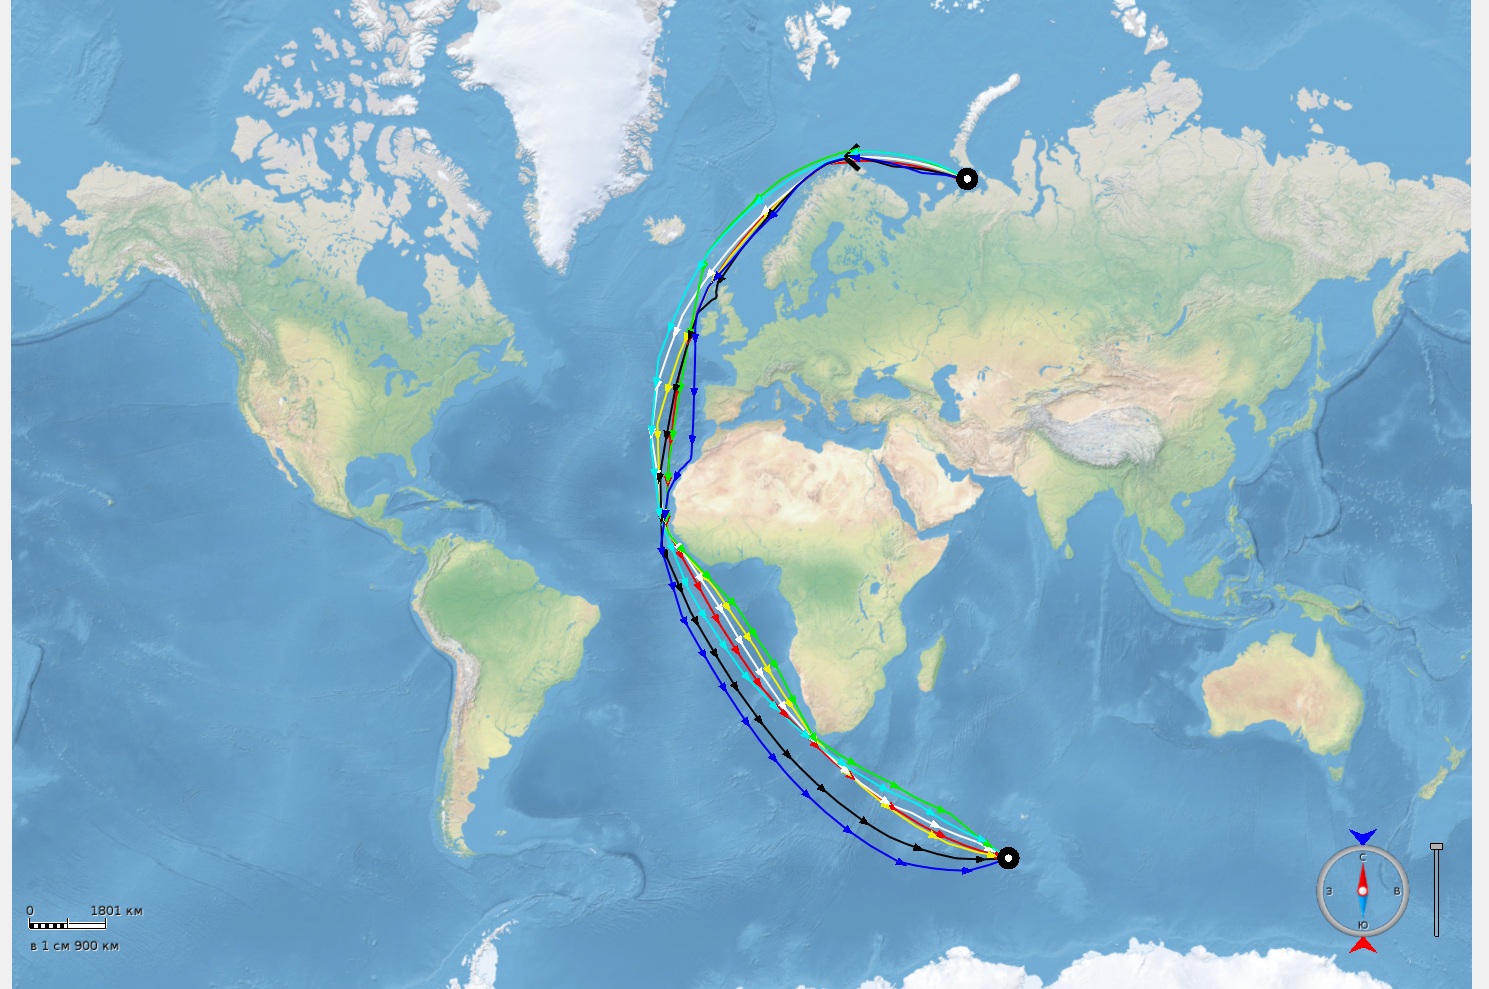
\includegraphics[width=\textwidth, clip=true, trim = 600 0 0
    0]{Introduction/existing-bad}
    \caption{Маршруты, найденные алгоритмом~\cite{lim2005shortest}}
    \label{fig:limkim1}
\end{figure}

\newcommand{\limkimpicture}[1] {
    \begin{center}
    \includegraphics[height=.4\textheight, clip=true, trim = 400 100 400
    40]{Introduction/#1}
    \end{center}
}

\begin{figure}
    \limkimpicture{limkim-only-one}
    \caption{Алгоритмом~\cite{lim2005shortest} найден лишь один маршрут}
    \label{fig:limkim2}
\end{figure}

\begin{figure}
    \limkimpicture{limkim-desired}
    \caption{Желаемые маршруты}
    \label{fig:limkim3}
\end{figure}

В статье приведён пример, демонстрирующий, что для графа дорог данное
решение действительно находит непохожие пути. Однако при поиске
семейств маршрутов в навигационном графе, построенном по полигональным
препятствиям, недостаточно в качестве критерия, описывающего похожесть
маршрутов, рассматривать лишь степень перекрытия.
Рисунок~\ref{fig:limkim1} демонстрирует это. На рисунке представлено
семь маршрутов, и нетрудно видеть, что любые два из них практически не
имеют общих рёбер, то есть степень перекрытия действительно очень
низкая. Однако все эти маршруты идут по одним и тем же морям и
океанам, поэтому такие маршруты нельзя назвать непохожими. Второй
недостаток данного подхода в том, что он находит слишком мало
маршрутов. Например, на рисунке~\ref{fig:limkim2} показана ситуация, в
которой данный алгоритм нашёл лишь маршрут через Панамский канал,
тогда как хотелось бы видеть альтернативный маршрут через южную часть
Южной Америки (рисунок~\ref{fig:limkim3}). Это связано с тем, что
после увеличения весов рёбер только на найденном маршруте следующий
путь зачастую будет проходить очень близко к предыдущему, из-за чего
алгоритм может сразу же прекратить работу.

\FloatBarrier

\subsection{Dijkstra-Hyperstar}

\label{subsec:dijkstra-hyperstar}

В статье~\cite{mafast} описываются три алгоритма поиска нескольких
маршрутов в графе, ориентированные на поиск путей в транспортных
сетях. Данные алгоритмы приводят к похожим результатам и различаются в
основном производительностью. Для анализа был выбран ASF (Adapted
Spiess and Florian) алгоритм. В данном алгоритме каждое ребро графа
помимо веса имеет некоторую частоту, которая соответствует тому, как
часто ходит транспорт по этому ребру, поэтому напрямую он не может
быть применён к задаче поиска семейств маршрутов по воде. Обратная
величина частоты соответствует максимальному времени ожидания
транспорта. Для исследования данного алгоритма частоты присваивались
случайным образом, чтобы максимальное время ожидания было того же
порядка, что и веса рёбер. В результате данный алгоритм присваивает
каждому ребру вероятность быть использованным в итоговом множестве
маршрутов.

После присвоения вероятностей рёбрам необходимо построить сами
маршруты. Для этого запускается случайный процесс, который на каждом
шаге по текущей вершине выбирает следующую в зависимости от
вероятностей, присвоенных исходящим рёбрам. Процесс начинается в
стартовой вершине и заканчивается при достижении целевой точки. Если
все исходящие рёбра имеют нулевую вероятность, то путь не может быть
найден и алгоритм заканчивает свою работу, иначе процесс повторяется,
пока не будет найдено максимальное число маршрутов или два одинаковых
маршрута.

\begin{figure}
    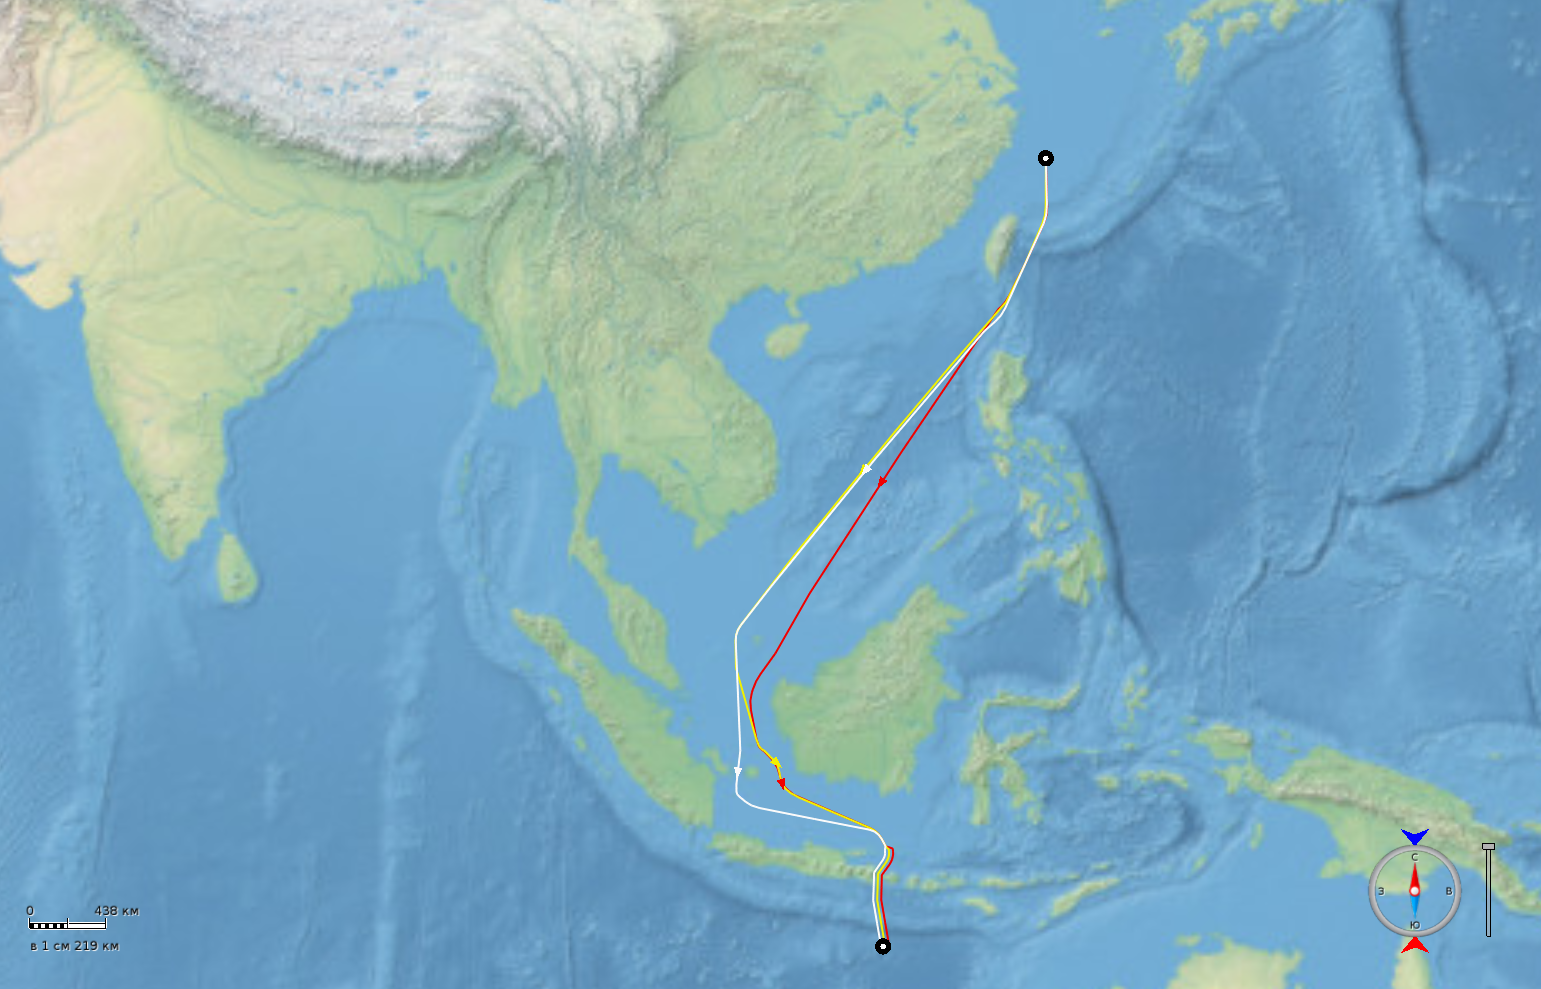
\includegraphics[width=\textwidth, clip=true, trim = 300 0 300
    0]{Introduction/hyperstar-example}
    \caption{Пример маршрутов, найденных ASF алгоритмом}
    \label{fig:asf}
\end{figure}

Главным минусом данного алгоритма является необходимость присвоения
частот рёбрам. Если все частоты равны, то алгоритм присваивает нулевую
вероятность всем рёбрам, не принадлежащим кратчайшему пути. Именно от
частот зависит то, насколько различны будут итоговые маршруты. Также
сам по себе алгоритм лишь находит вероятности рёбер, а значит,
построению маршрутов с его использованием в любом случае будет
свойственна недетерминированность. В большинстве же случаев маршруты
получаются похожими (например, рис.~\ref{fig:asf}).

\FloatBarrier

\section{Формальная постановка задачи}

\label{sec:formal-task}

На основе проведённого обзора и неформальных требований можно
формализовать постановку задачи. Дано множество полигональных
препятствий $C$, начальная точка $S$ и конечная точка $D$. По
полигональным препятствиям строится навигационный граф. Требуется
найти множество путей $P$ из точки $S$ в точку $D$, удовлетворяющих
следующим свойствам:
\begin{itemize}
  \item Каждый путь $p \in P$ представлен ломаной, любой отрезок
    которой не пересекает ни один контур из $C$.
  \item Пусть $q$ --- кратчайший путь. Обозначим как $len(p)$ длину пути $p$.
    Тогда $\forall p \in P: len(p) < C_0 \cdot len(q)$, где $C_0 > 1$
    является параметром задачи.
  \item Любыe два пути $p, q \in P$ не являются похожими в смысле
    критерия, сформулированного ниже.
\end{itemize}

Для определения похожести маршрутов используются две метрики,
заданные на множестве маршрутов:
\begin{equation*}
    \rho_1 (P, Q) = \max(\max_{u \in P} \min_{v \in Q} \rho_g(u,
    v), \max_{v \in Q} \min_{u \in P} \rho_g(u, v))
\end{equation*}

$\rho_g(u, v)$ означает длину кратчайшего пути в навигационном графе
между вершинами $u$ и $v$. В данной метрике для каждой вершины
маршрута рассматривается длина кратчайшего пути до второго маршрута.
Значением метрики является максимум всех таких длин. Большое значение
этой метрики означает, что для какой-то вершины кратчайший путь в
навигационном графе до второго маршрута имеет большую длину, что
является хорошим показателем того, что маршруты непохожи.
\begin{equation*}
    \rho_2 (P, Q) = \max(\max_{u \in P} \frac{\min\limits_{v \in Q_u}
    \rho_g(u, v)}{\min\limits_{v \in Q_u} \rho_r(u, v)}, \max\limits_{v \in Q} \frac{\min\limits_{u \in P_v}
    \rho_g(u, v)}{\min\limits_{u \in P_v} \rho_r(u, v)})
\end{equation*}
\begin{equation*}
    P_v = \{ u \in P : \rho_r(u, v) > \varepsilon \cdot len(P) \}
\end{equation*}
\begin{equation*}
    Q_u = \{ v \in Q : \rho_r(u, v) > \varepsilon \cdot len(Q) \}
\end{equation*}

$\rho_r(u, v)$ означает расстояние между $u$ и $v$ в мире. Данная
метрика аналогична первой, однако максимум берётся не по длинам
кратчайших расстояний в графе, а по отношению длины кратчайшего
расстояния в графе к расстоянию до ближайшей вершины в мире. Большое
значение этой метрики означает, что для какой-то вершины длина кратчайшего
пути в навигационном графе до второго маршрута существенно больше, чем
кратчайшее расстояние в мире. Это является показателем того, что между
маршрутами имеется препятствие. При этом не рассматриваются пары
слишком близких вершин, поскольку между ними может быть препятствие
очень небольших размеров, которое не делает маршруты непохожими,
однако делает значение метрики большим. Число $\varepsilon$ также
является параметром алгоритма.

На основании этих двух метрик формируется следующий критерий
похожести маршрутов $P$ и $Q$.
\begin{itemize}
  \item Если $\rho_1(P, Q) > C_{1max} \cdot \min(len(P), len(Q))$, то
    маршруты являются непохожими.
  \item Если $\rho_1(P, Q) < C_{1min} \cdot \min(len(P), len(Q))$, то
    маршруты являются похожими.
  \item Если ни один из первых двух пунктов не выполнен и $\rho_2(P,
    Q)$ > $C_2 \cdot \min(len(P), len(Q))$, то маршруты являются непохожими.

  \item В противном случае маршруты являются похожими.
\end{itemize}

Константы $C_{1max}$, $C_{1min}$, $C_2$ также являются параметрами. В
работе использовались следующие значения параметров, подобранные в результате экспериментов:

$C_0 = 2,5$; $C_{1max} = 0,5$; $C_{1min} = 0,2$; $C_2 = 1,15$;
$\varepsilon = 0,1$.

\begin{figure}
    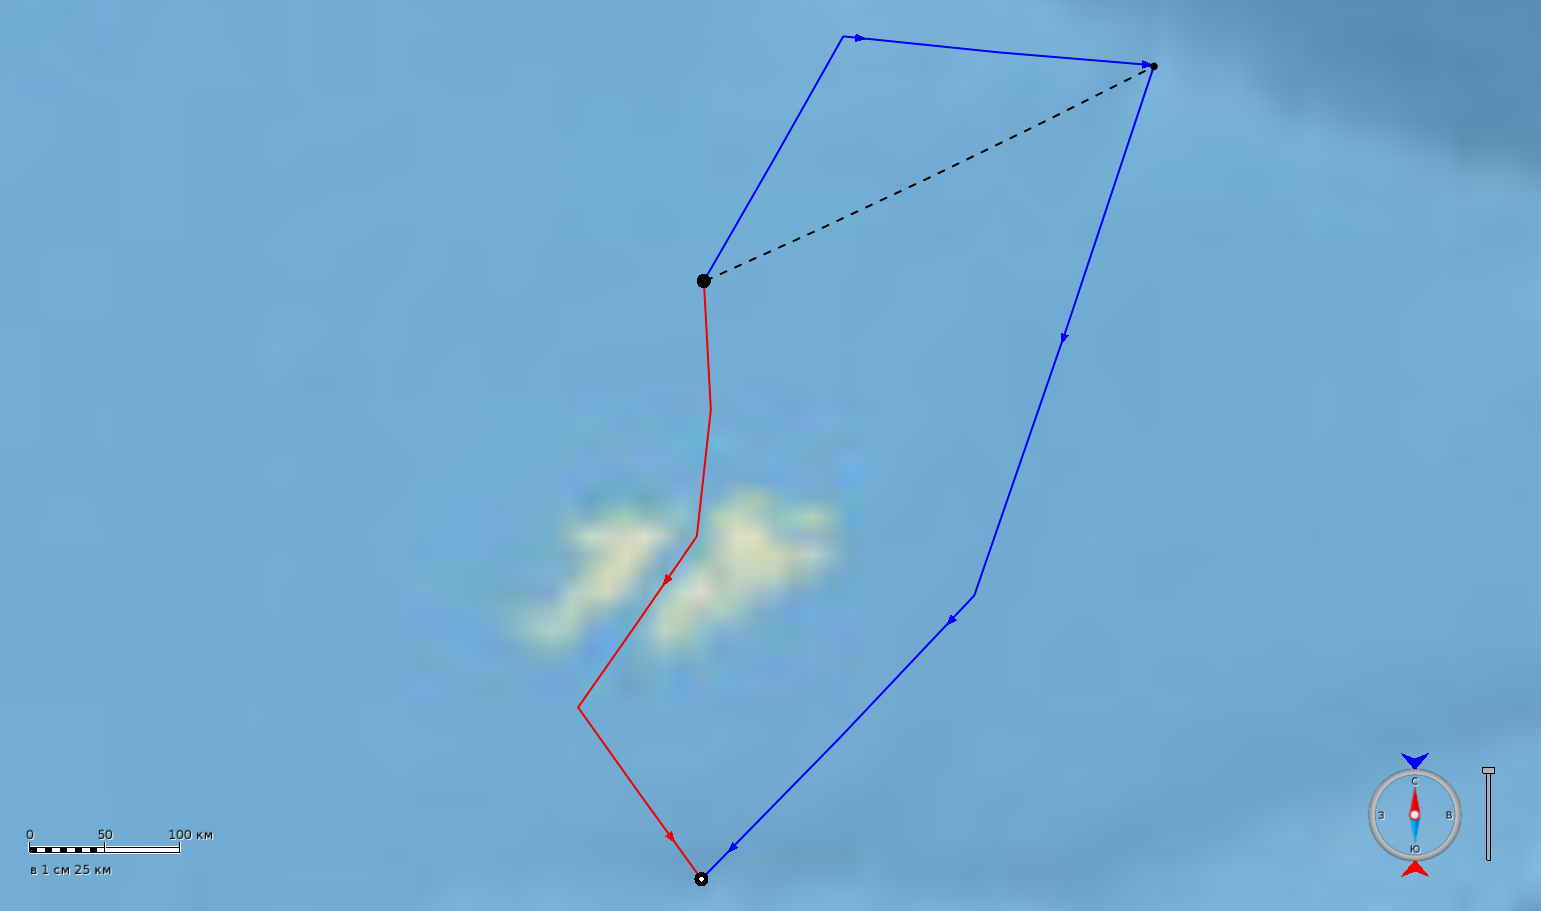
\includegraphics[width=\textwidth]{Solution/metrics/1-dissimilar}
    \caption{Маршруты непохожи по первой метрике}
    \label{fig:1-dissimilar}
\end{figure}

На рисунке~\ref{fig:1-dissimilar} изображены два маршрута (синий и
красный). Чёрная пунктирная линия соединяет две вершины, на которых
достигается значение первой метрики (339 км). При этом длина красного
маршрута составляет 435 км. Поскольку $\frac{339}{435} = 0,78 > 0,5$,
то маршруты считаются непохожими.

\begin{figure}
    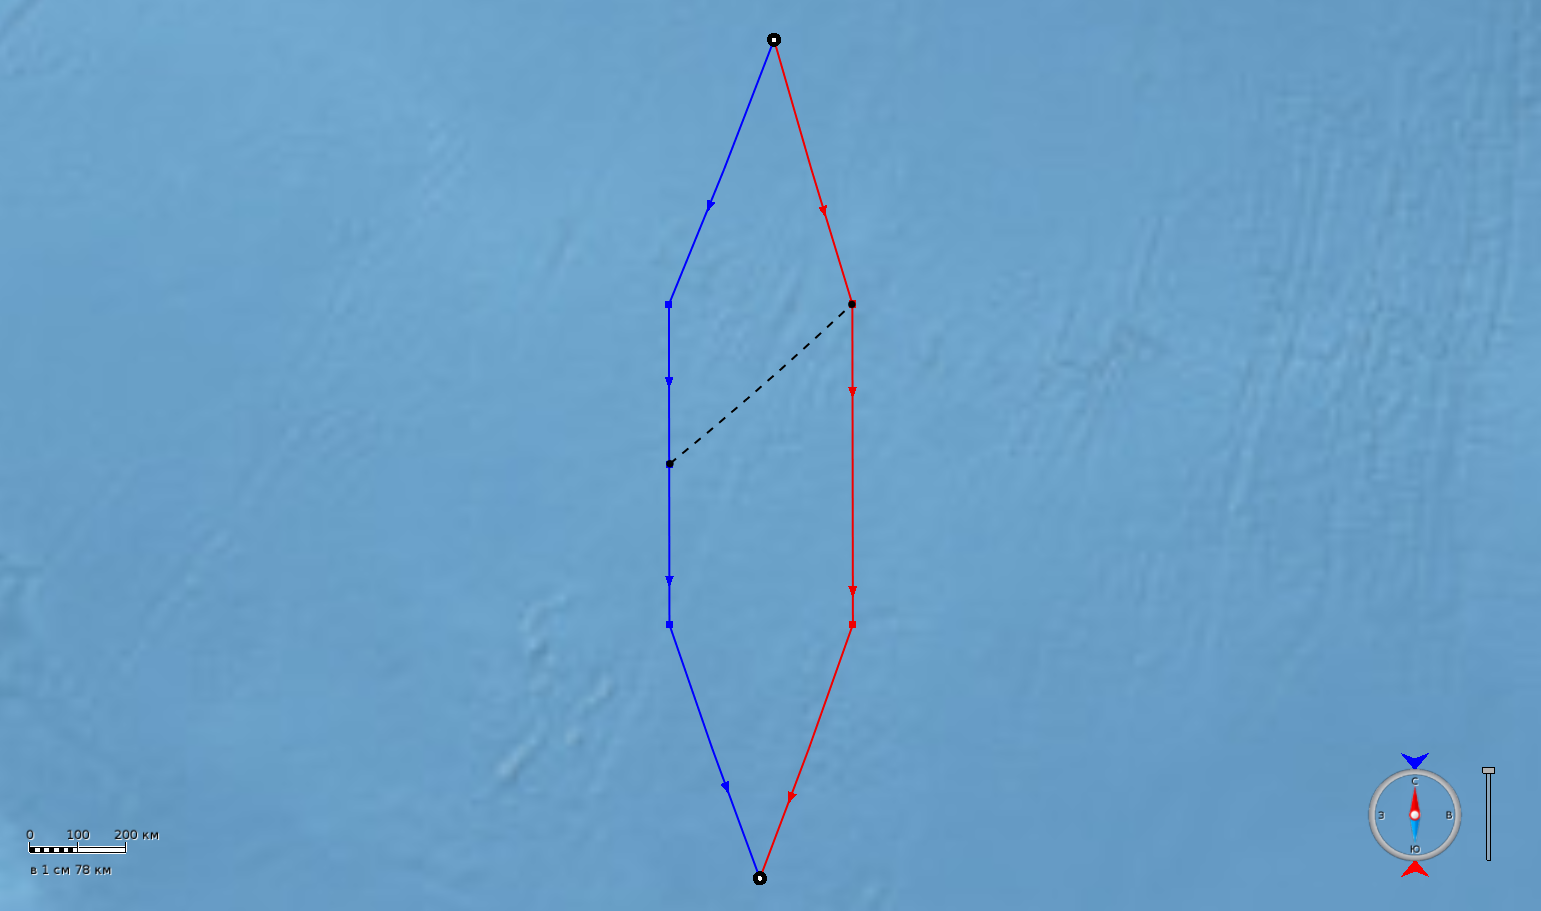
\includegraphics[width=\textwidth]{Solution/metrics/1-uncertain-2-similar}
    \caption{Маршруты похожи по второй метрике}
    \label{fig:1-uncertain-2-similar}
\end{figure}

Для маршрутов, изображённых на
рисунке~\ref{fig:1-uncertain-2-similar}, значение первой метрики равно
502 км, а длина кратчайшего из двух маршрутов равна 1704 км. $0,2 <
\frac{502}{1704} = 0,29 < 0,5$, поэтому используется значение второй метрики.
Поскольку между каждой парой вершин на маршрутах не имеется
препятствий, то значение этой метрики равно 1. Таким образом, эти два
маршрута считаются похожими.

\begin{figure}
    \centering
    \begin{minipage}{.5\textwidth}
        \centering
        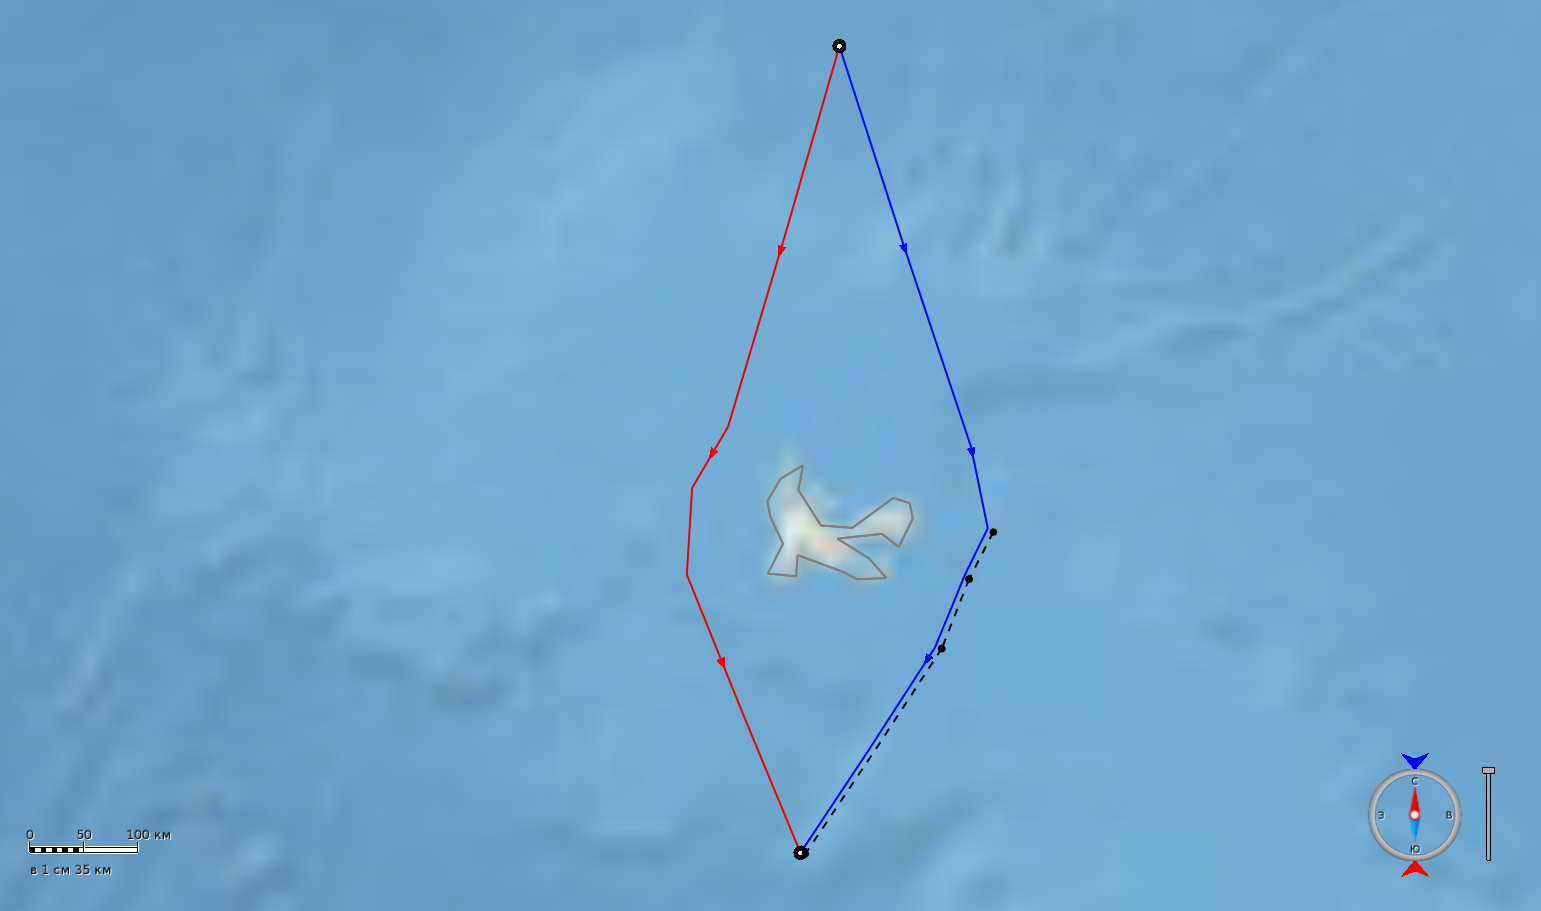
\includegraphics[width=\textwidth, clip=true, trim = 300 0 300
        0]{Solution/metrics/1-uncertain-2-dissimilar-gclosest}
        \captionof{figure}{Маршруты «возможно, похожи» по первой метрике\dots}
        \label{fig:1-uncertain-2-dissimilar-gclosest}
    \end{minipage}%
    \begin{minipage}{.5\textwidth}
        \centering
        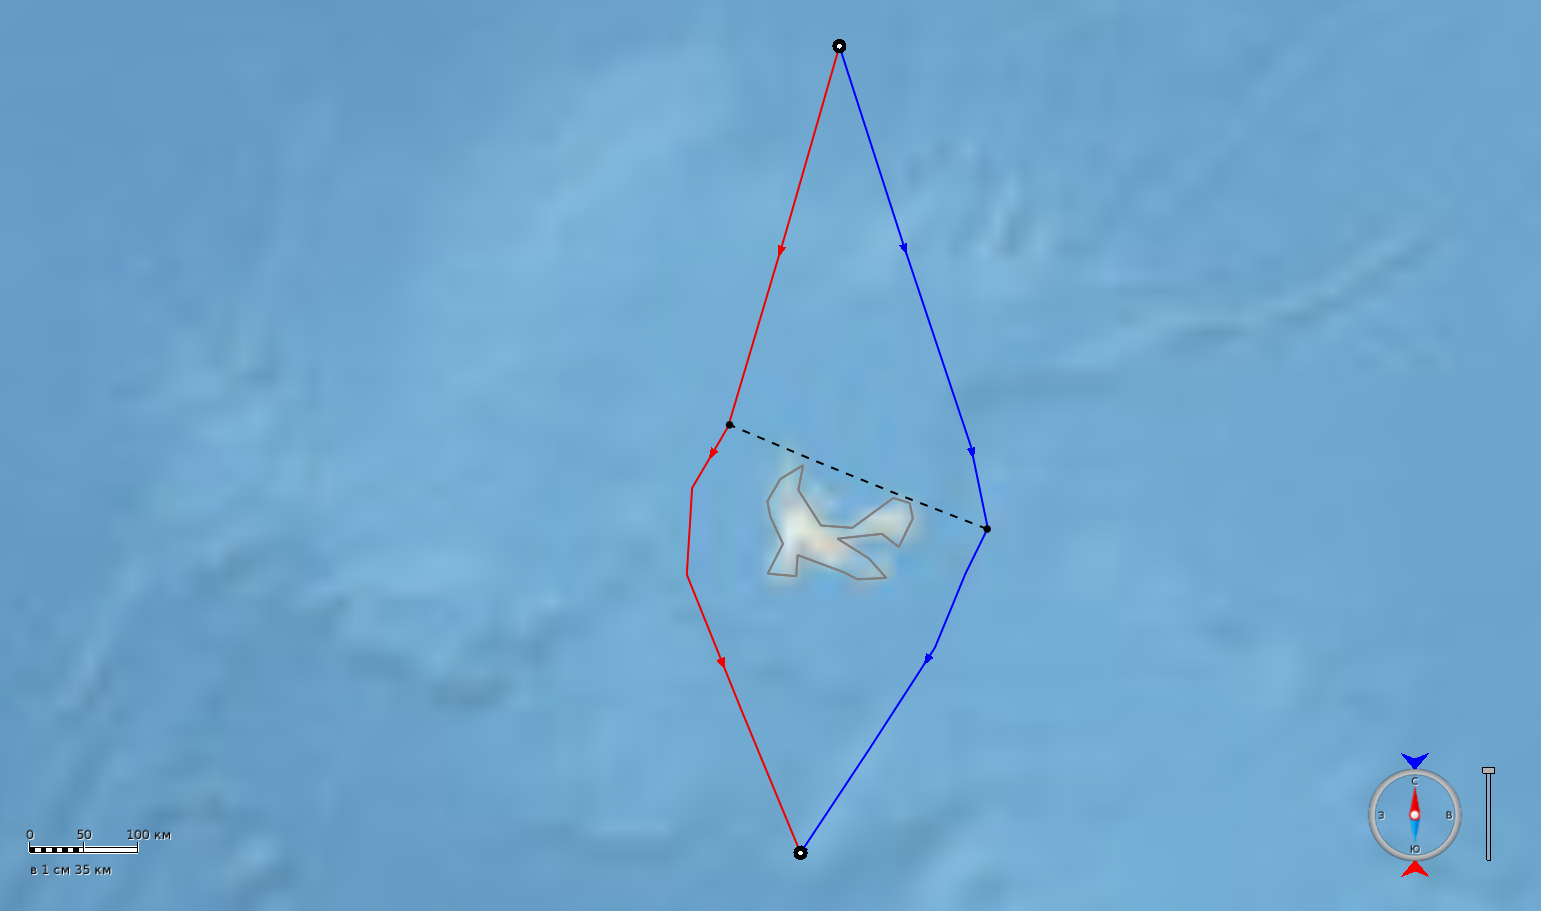
\includegraphics[width=\textwidth, clip=true, trim = 300 0 300
        0]{Solution/metrics/1-uncertain-2-dissimilar-closest}
        \captionof{figure}{\dots и точно непохожи по второй из-за
          острова между ними.}
        \label{fig:1-uncertain-2-dissimilar-closest}
    \end{minipage}
\end{figure}

Для маршрутов, изображённых на рисунках
\ref{fig:1-uncertain-2-dissimilar-gclosest} и
\ref{fig:1-uncertain-2-dissimilar-closest}, значение первой метрики
равно 307 км (на первом рисунке пунктиром показано, для каких двух
точек оно достигается). Длина кратчайшего из двух маршрутов равна 814
км. $0,2 < \frac{307}{814} = 0,38 < 0,5$, поэтому в данном случае тоже
используется вторая метрика. На втором рисунке пунктиром показана
ближайшая вершина второго пути для той же вершины первого. Расстояние
до неё составляет 251 км. Значение второй метрики достигается между
теми же двумя вершинами и равно $\frac{307}{251} = 1,22 > 1,15$. Поэтому
данные два маршрута считаются непохожими, что полностью согласуется с
неформальными требованиями, описанными ранее.

\begin{figure}
    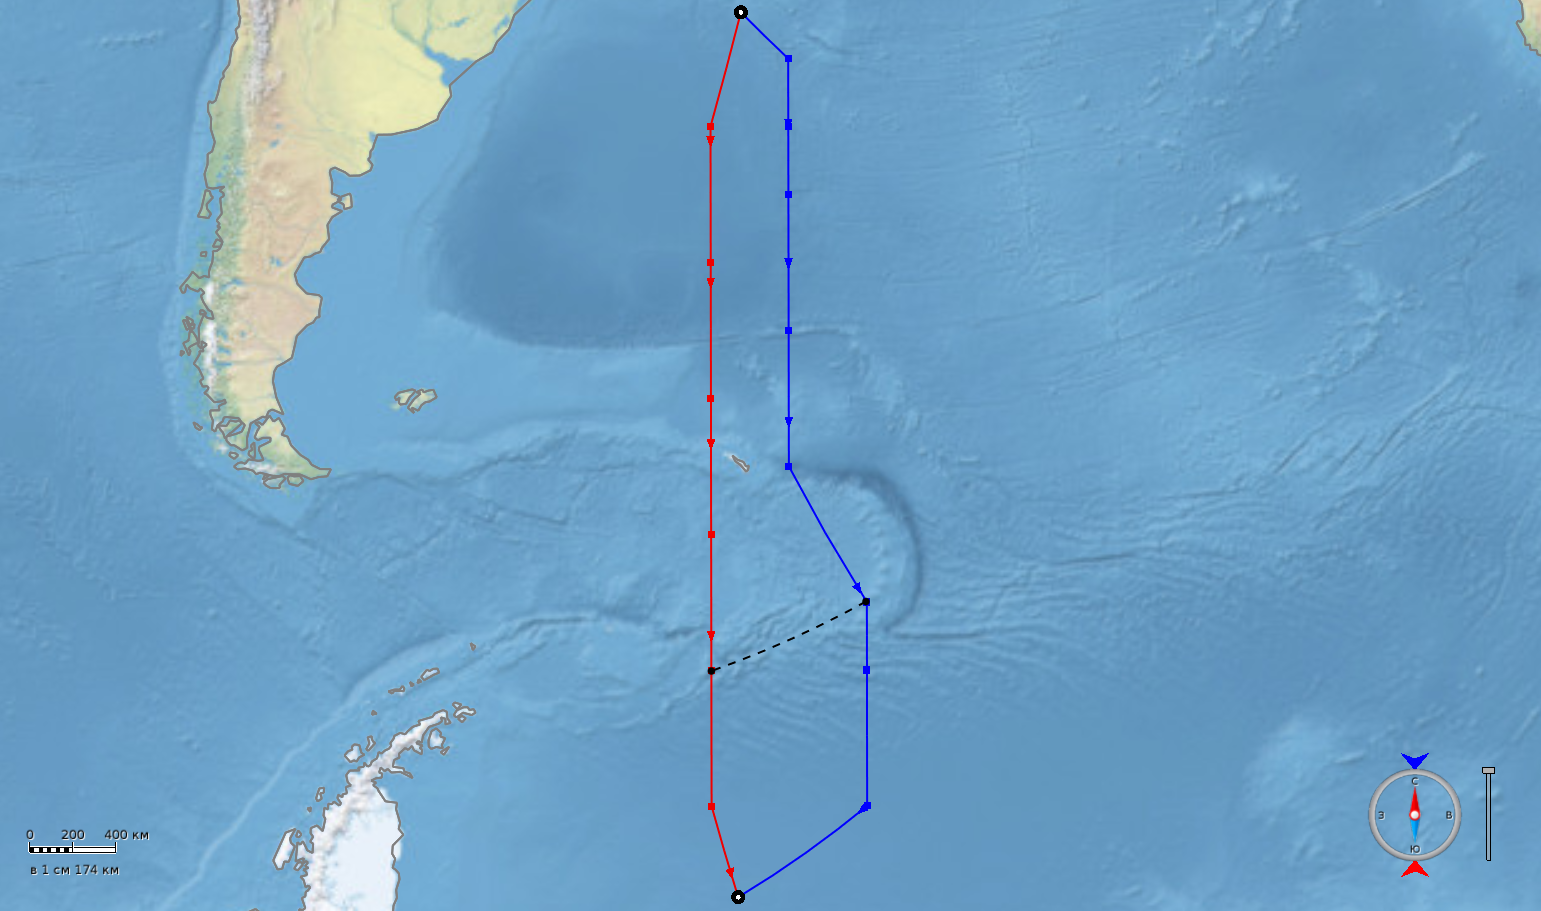
\includegraphics[width=\textwidth]{Solution/metrics/1-similar}
    \caption{Маршруты похожи по первой метрике}
    \label{fig:1-similar}
\end{figure}

Наконец, на рисунке~\ref{fig:1-similar} представлены маршруты, для
которых значение первой метрики составляет 641 км, а длина кратчайшего
из них --- 4059 км. Таким образом, поскольку $\frac{641}{4059} = 0,16
< 0,2$, то эти маршруты считаются похожими по первой метрике. Хоть
между ними и имеется препятствие, его размеры пренебрежимо малы,
поэтому логично считать такие маршруты похожими.

\FloatBarrier

